\section{问题二：异构无人机多航次运输与资源调度}

问题一在“每架次仅服务一个服务区、且忽略实体机与共享电池”的条件下给出了运输能力和组批基准。问题二在相同飞行物理模型上允许单架次访问多个服务区，并要求把80个货箱落实到8架实体运输无人机与14组共享电池上，同时满足配送时限。货箱划分、访问顺序、机型、机体、电池和起飞时刻由此相互耦合：路线决定能耗与到达时刻，到达时刻决定时限是否满足，能耗和充电时间又影响机体与电池的后续复用。

\subsection{问题分析与建模框架}

本问沿用第2、3章的物理口径：航段以两节点水平直线为投影，巡航海拔取沿线DEM最高地面以上50~m，交接后从该站作业高度重新爬升；航段飞行时间与能耗按式~\eqref{eq:range}--\eqref{eq:energy}计算；每个架次总耗电不超过$(1-\rho_g)E_g^{\rm use}$，货箱不可拆分且逐站扣重。相对问题一，本问新增三类决策与约束：访问顺序成为决策变量，单架次可服务多个服务区；运输任务需要落实到具体机型、机体和电池的占用日历；配送时限分为硬截止与软期望时刻。硬截止集合包含31箱，软迟到集合包含64箱非医疗物资，两者允许重叠。

由此带来三个难点。{\heiti 一是组合规模}：80个不可拆货箱需要同时决定航次划分、访问顺序、机型、实体机、电池和起飞时刻，决策之间存在明显耦合。{\heiti 二是资源时序约束}：电池遵循“使用—充电—再用”（等效充满时间对A、B、C型分别为1800、2400、3000~s），机体另受准备300~s与逐箱装载30~s约束，因此架次之间不能独立安排。{\heiti 三是指标量纲不同}：硬截止决定方案是否可行，及时性、收尾、能耗、架次数和能源裕度则承担不同的评价作用，不宜直接加权为单一分数。

针对上述难点，本文采用三层框架。物理层将航程、能耗、交接与充电规则写成路线成本函数；模型层以0--1变量、连续时间和资源区间完整描述货箱分配、路径、机型、资源与时间约束；算法层采用“路线生成—固定路线调度”的分层方法，在给定搜索预算内比较候选。该模型是混合离散—连续约束模型，不将含可选区间和\texttt{NoOverlap}约束的完整描述称为标准混合整数线性规划。完整模型用于说明可行域和指标，实际方案由分层算法产生，并另行进行约束回代验证。

\subsection{配送时限与优化指标}

本问沿用第 4 章符号，不重复定义公共符号，只在首次出现处补充航段序号 $k$、架次总耗时 $\Delta_p$、货箱自起飞至交接完成的时间 $\tau_{pb}$ 与优先加权平均送达时刻 $\bar{T}^{\rm arr}_\omega$。在完整模型中，$p$ 表示潜在航次；实际算法中，一条路线由箱集、访问顺序和机型共同确定，记为 $p=(B_p,\pi_p,g_p,E_p,\Delta_p,\{\tau_{pb}\})$。

\subsubsection{硬截止与软迟到集合}

每个货箱 $b$ 在附件中可能同时带有期望送达时刻 $T_b$ 与首批截止时刻 $f_b$。出于救援优先级考虑，本文按“就紧”原则生成其适用硬截止：

\begin{equation}
D_b=
\begin{cases}
\min(T_b,f_b), & b\ \text{兼属医疗与首批},\\
T_b, & b\ \text{仅属医疗},\\
f_b, & b\ \text{仅属首批},\\
+\infty, & \text{其他},
\end{cases}
\qquad T_b^{\rm arr}\le D_b\quad (b\in\mathcal{H}).
\label{eq:q2-deadline}
\end{equation}

按附件逐箱清单统计，80 箱的构成与时限归属如表~\ref{tab:box-composition} 所示。首批保障货箱共 30 箱，由 15 箱医疗物资与 15 箱饮用水构成；其中 15 箱医疗物资已计入医疗集合，故去重后受硬截止约束的货箱为 $16+30-15=31$ 箱。是否兼属直接决定取较早时刻，这一处理避免了同一箱在两套时限下出现宽松解释；按同一清单重算，80 箱合计 758~kg、2.011~m$^3$，与附件汇总值一致，说明时限表与逐箱清单位于同一口径下。

\begin{table}[htbp]
\centering
\caption{货箱型构成与时限归属}
\label{tab:box-composition}
\small
\setlength{\tabcolsep}{3pt}
\begin{tabular}{lccccc p{1.7cm}}
\toprule
{\heiti 物资类型} & {\heiti 箱数} & {\heiti 单箱质量/kg} & {\heiti 单箱体积/m}$^3$ & {\heiti 优先系数} & {\heiti 首批箱数} & {\heiti 是否受硬截止} \\
\midrule
医疗物资 & 16 & 3 & 0.012 & 24/22/20/16 & 15 & 是（期望时刻） \\
饮用水 & 36 & 14 & 0.027 & 12/10/8 & 15 & 是（首批截止） \\
应急食品 & 19 & 8 & 0.028 & 10/8/6 & 0 & 否 \\
生活卫生用品 & 9 & 6 & 0.035 & 8/6/4 & 0 & 否 \\
\midrule
合计 & 80 & --- & --- & --- & 30 & 去重后 31 \\
\bottomrule
\end{tabular}
\end{table}

所有64箱非医疗物资的期望送达时刻均进入软指标，其中包括15箱同时受首批硬截止约束的饮用水。换言之，这15箱既要满足首批截止，也按各自期望时刻计算软迟到；16箱医疗物资的期望时刻已经作为硬截止，不再重复计入软迟到。非医疗货箱的迟到量定义为

\begin{equation}
L_b=\max\bigl(0,\;T_b^{\rm arr}-T_b\bigr).
\label{eq:q2-late}
\end{equation}

全部非医疗箱的加权迟到 $\bar{L}_\pi=\sum_{b\notin\mathcal{M}}\omega_bL_b$ 是及时性指标，见式~\eqref{eq:q2-metrics}。其中 $\omega_b$ 取附件给出的应急优先系数：饮用水为12、10或8，应急食品为10、8或6，生活卫生用品为8、6或4。医疗物资的优先系数只用于加权送达时刻，不进入软迟到。硬截止本身不设权重，一旦违反即判方案不可行。

\subsubsection{决策变量与指标分类}

完整模型以 $a_p$、$x_{bp}$、$h_{pi}$、$v_{pij}$ 表示航次启用、箱分配、服务区访问与路径弧，以 $y_{pg}$、$z_{pu}$、$w_{pr}$ 表示机型、实体机与电池的三层指派，并引入架次开始时刻 $s_p$、返航结束时刻 $e_p$ 与架次能耗 $E_p$。在此基础上定义加权迟到、收尾时间、优先加权平均送达时刻和总能耗：

\begin{equation}
\bar{L}_\pi=\sum_{b\notin\mathcal{M}}\omega_bL_b,\qquad
C_T=\max_{p}e_p,\qquad
\bar{T}^{\rm arr}_\omega=\frac{\sum_b\omega_bT_b^{\rm arr}}{\sum_b\omega_b},\qquad
E_T=\sum_{p}E_p,
\label{eq:q2-metrics}
\end{equation}

以及刻画方案离能量上限还有多远的最小能源裕度

\begin{equation}
\gamma_E=\min_{p:\,a_p=1}\frac{(1-\rho_{g_p})E_{g_p}^{\rm use}-E_p}{E_{g_p}^{\rm use}}.
\label{eq:q2-margin}
\end{equation}

这些量的作用分为四层。第一，货箱唯一分配、物理能力、31箱硬截止及机体和电池不冲突共同决定可行性。第二，在硬可行之后，正式比较依次考察加权迟到$\bar{L}_\pi$、收尾时间$C_T$、优先加权平均送达$\bar{T}^{\rm arr}_\omega$、总能耗$E_T$和架次数$N_T$。第三，$\gamma_E$用于报告不同机型架次相对返航储备下限的最小裕度，不替代能量可行性约束。第四，能耗、架次和稳健性排序仅用于补充目标剖面实验，并在迟到与收尾容忍约束下改变后续指标的优先级。各层均采用约束或字典序比较，不把不同量纲的指标加权求和。

\subsection{多航次运输与资源约束模型}

该问题可表示为带时间窗和共享资源的异构多航次路径问题。以下六类约束共同描述货箱分配、路径、机型、载荷、时间与资源周转，其中$p$表示候选航次。

{\heiti（1）箱分配与访问一致性。}
\begin{equation}
\sum_p x_{bp}=1,\qquad
x_{bp}\le a_p,\qquad
x_{bp}\le h_{p,a(b)},\qquad
h_{pi}\le\sum_{b:\,a(b)=i}x_{bp}.
\label{eq:q2-assign}
\end{equation}
第一式对应货箱不可拆分；第二式保证只有已启用航次才能承运；第三式使箱分配以其目的服务区被访问为前提；第四式排除访问某服务区却无箱可交的空访问，从而保证访问变量与货箱分配保持一致。

{\heiti（2）路径流守恒与子回路消除。}
\begin{align}
&\sum_{j\in N}v_{p0j}=a_p=\sum_{i\in N}v_{pi0},\qquad
\sum_j v_{pij}=h_{pi}=\sum_j v_{pji},\nonumber\\
&o_{pi}-o_{pj}+|N|v_{pij}\le|N|-1+|N|\bigl(2-h_{pi}-h_{pj}\bigr).
\label{eq:q2-route}
\end{align}

第一行要求每个航次以 O01 为起点与终点、每个被访问站入弧数等于出弧数等于 1，即为一条简单回路；第二行是 Miller--Tucker--Zemlin 型次序约束，当弧 $i\to j$ 被使用且两站均被访问时强制 $o_{pj}\ge o_{pi}+1$，排除与 O01 脱离的小回路。由于本题允许一架次访问多站，若不显式消除子回路，求解器极易把多条互不相连的短回路误判为可行。

{\heiti（3）机型、机体与电池的三层指派。}
\begin{equation}
\sum_g y_{pg}=a_p,\qquad
\sum_{u\in\mathcal{U}_g}z_{pu}=y_{pg},\qquad
\sum_{r\in\mathcal{Q}_g}w_{pr}=y_{pg},
\label{eq:q2-resource}
\end{equation}

即每个启用航次恰选一种机型，所用实体机与电池都必须属于该机型（$\mathcal{U}_g$、$\mathcal{Q}_g$ 分别为机型 $g$ 的实体机集合与共享电池集合）。这使得题面“同一机型电池可跨机调度、不同机型不可混用”被写成下标约束，是离散资源在模型中的唯一入口。

{\heiti（4）载重、容积与逐段载荷。}
\begin{equation}
\sum_b M_bx_{bp}\le\sum_g Q_gy_{pg},\qquad
\sum_b V_bx_{bp}\le\sum_g V_gy_{pg},\qquad
E_p\le\sum_g(1-\rho_g)E_g^{\rm use}y_{pg}.
\label{eq:q2-capacity}
\end{equation}

前两式作用于整个航次的箱集而非单站箱集，因为多站架次的载重峰值出现在尚未交付任何箱的起飞时刻；第三式把“同一路线换用不同机型是否仍安全”直接写进约束。与之配套，逐段剩余载荷按尚未交付箱重之和更新：
\begin{equation}
q_p^{k}=\sum_{\substack{b:\,x_{bp}=1,\ a(b)\in\pi_p\ \text{中第}\ k\ \text{段及之后}}}\!\!M_b,
\label{eq:q2-payload}
\end{equation}
其中 $k$ 为航段序号、$\pi_p$ 为访问序列，即每交付一站立即扣重，再以更轻载荷计算后续航段。

{\heiti（5）时间推进。}令 $e_p=s_p+\Delta_p$，并在 $x_{bp}=1$ 时强制 $T_b^{\rm arr}=s_p+\tau_{pb}$，其中 $\Delta_p$ 为架次总耗时、$\tau_{pb}$ 为该箱自起飞至交接完成的时间。站点交接时间按基础交接加逐箱增加计（A、B 型 $150+30n_i$~s，C 型 $180+36n_i$~s，$n_i$ 为交接箱数），本站全部货箱统一记为交接结束时刻，于是
\begin{equation}
t_{p,i+1}=t_{p,i}+\bigl(t^{\rm hand}+n_it^{\rm box}\bigr)+t^{g_p}_{i,i+1},
\label{eq:q2-time}
\end{equation}
其中 $t^{g}_{i,i+1}$ 为式~\eqref{eq:energy}同组的航段飞行时间。本站全部货箱统一记为交接结束时刻送达。实际逐箱交付可能在交接过程中提前完成，因此这一记账方式不会夸大时限裕度，是一种保守处理。

{\heiti（6）机体与电池的周转闭合。}同一架实体机与同一组电池都要被多个航次复用，故对每架机体、每组电池设置以 $z_{pu}$、$w_{pr}$ 为存在变量的可选区间并施加 NoOverlap：
\begin{equation}
[s_p,\,e_p)\ \text{两两不重叠}\ (u\ \text{相同}),\qquad
\bigl[s_p,\ e_p+t^{\rm chg}_{g_p}\bigl(1-E_p/E^{\rm use}_{g_p}\bigr)\bigr)\ \text{两两不重叠}\ (r\ \text{相同}).
\label{eq:q2-turnover}
\end{equation}
电池区间被延长至充满，因为再次投入前须恢复 100\%，而充电时段同样占用该组件。由于 $t^{\rm chg}$ 取决于任务结束时的荷电状态，而荷电状态又由架次能耗决定，充电时长与路线能耗相互关联。本文采用可选区间变量与 NoOverlap 约束描述机体、电池及充电周转；早返航的机体会为后续架次留出更多复用时间。

式~\eqref{eq:q2-assign}--\eqref{eq:q2-capacity}、\eqref{eq:q2-payload}、\eqref{eq:q2-time}和\eqref{eq:q2-turnover}共同给出本问的完整约束描述。若将路线选择、逐段载荷、连续时刻和全部资源区间同时放入一个模型，以30个候选航次估算，仅$v_{pij}$就约有$30\times16\times16\approx7.7\times10^3$个，$x_{bp}$约有$2.4\times10^3$个，此外还包含三层指派变量与资源区间。由于路线决定能耗和充电时长，离散路径与资源周转相互关联，本文不直接求解这一整体模型，而是按路线生成与资源调度两个子结构分层处理。

\subsection{路线生成与固定路线调度方法}

给定运输路线后，资源排程可作为独立子问题求解，因此本文将路线生成与实体资源调度分层处理。给定一条完整路线——箱集 $B_p$、访问序列 $\pi_p$、机型 $g_p$ 及其决定的 $\Delta_p$、$E_p$ 与 $\{\tau_{pb}\}$——剩余问题是为该航次安排开始时刻并分配机体与电池，变量规模显著降低，可由约束规划求解。上层搜索负责路线组合，下层求解负责时间与资源分配，接口为：

\begin{itemize}
  \item 上层输出：完整路线列 $p=(B_p,\pi_p,g_p,E_p,\Delta_p,\{\tau_{pb}\})$；
  \item 下层输入：该路线列与机体、电池日历；
  \item 下层输出：开始时刻 $s_p$、机体 $u_p$、电池 $r_p$，以及 $e_p=s_p+\Delta_p$ 与 $T_b^{\rm arr}=s_p+\tau_{pb}$。
\end{itemize}

下层若在给定时间内找到满足资源日历和硬时限的排程，则将其作为该路线组合的可行排程；若求解器明确返回不可行，则剔除该组合；若时间保护内未得到可接受状态，也不据此声称已经证明不可行。上层路线由随机化构造（独立重建方案）和共享五类邻域的局部改造产生：调整航次次序、整箱跨航次搬移、单箱拆成直送、更换机型或重排站序、合并两个航次。每次变换均重新检查载重、容积和能量；搜索过程中由顺序解码生成暂定资源日历并计算硬截止违反数，入选的路线组合再交给CP-SAT调度和独立验证。三种局部搜索共用这些邻域而采用不同接受准则：局部爬山每轮考察10个邻居、连续8轮无改进即回退；禁忌搜索每轮考察10个邻居、禁忌期限为12轮，并允许优于当前全局最好方案的候选破禁；模拟退火的最低温度为0.001，按已评估比例降温，并以0.02尺度归一化词典序相对损失。每次变换最多尝试35次，上述参数均来自实际运行配置。

下层在路线固定后只保留排程部分：
\begin{equation}
e_p=s_p+\Delta_p,\qquad
T_b^{\rm arr}=s_p+\tau_{pb},\qquad
\sum_{u\in\mathcal{U}_{g_p}}z_{pu}=1,\qquad
\sum_{r\in\mathcal{Q}_{g_p}}w_{pr}=1,
\label{eq:q2-schedule}
\end{equation}

即每条路线列恰占一架同型机体与一组同型电池。结合式~\eqref{eq:q2-turnover}的区间约束和式~\eqref{eq:q2-deadline}的硬截止，下层成为含资源日历与时间窗的排序问题，决策变量只包括开始时刻和两类资源编号。本文用CP-SAT在给定时间保护内求解这一子问题。

只有当求解状态为\texttt{OPTIMAL}时，才认为该次固定路线排程达到最优。只有当状态为\texttt{INFEASIBLE}时，才认为该排程子问题不可行。

正式主方案不依赖有限时状态作证明，而是另经逐箱、逐航次和逐资源回代确认可行。

\subsection{搜索实验与主方案选择}

四方法主实验比较随机化构造、局部爬山、模拟退火和禁忌搜索。每种方法使用10个随机种子，共40次运行；每个种子只独立构造一次初始方案，并由四种方法共享该起点。随机化构造作为独立方法时会在相同预算内反复重建方案，而其余三种方法从共享起点使用相同的五类邻域。每次运行最多评价30个有效候选，墙钟保护为90~s，固定路线排程保护为1.2~s。40次主实验统一采用及时性排序，即依次比较硬可行性、加权迟到、收尾时间、优先加权送达、能耗、架次数和能源裕度；全部运行均达到30次有效评估，且没有触发90~s墙钟保护。

除上述40次主实验外，另以局部爬山在相同10个种子和预算下分别进行能耗、架次数和能源裕度三个目标剖面，共30次补充运行。这些剖面将“加权迟到不超过对应初始方案、收尾时间不超过初始值的1.10倍”设为优先容忍条件，超出量先于剖面指标比较，再改变后续指标的优先顺序。补充运行用于观察指标权衡，不纳入表~\ref{tab:q2_formal_protocol}的四方法均值与标准差。

24架次方案来自此前将全部期望时刻按严格时限处理的归档实验，具体来源为局部爬山种子1。该方案没有参加本轮40次搜索，而是作为外部基线参与比较。按当前统一口径重新回放后，其指标为24架次、总能耗71.9169~kWh、收尾6276.83~s、优先加权平均送达45.69~min、加权迟到0、最低能源裕度0.004065。40次主实验均完成80箱配送且无硬截止违约，表~\ref{tab:q2_formal_protocol}给出四种方法在10个种子上的均值与标准差。

% Generated by code/generate_paper_tables.py; edit the source results, then regenerate.
\begin{table}[H]\centering\normalsize
\caption{同初始解下四种路线搜索的性能比较（均值±标准差，每法10个种子）}\label{tab:q2_formal_protocol}
\begin{tabular}{lrrrr}
\toprule
方法 & 可行运行 & 返航/min & 能耗/kWh & 架次\\\midrule
随机化构造 & 10/10 & 159.19$\pm$17.12 & 76.7629$\pm$2.1321 & 23.70$\pm$0.90\\
局部爬山 & 10/10 & 142.13$\pm$13.11 & 80.7906$\pm$3.9916 & 26.70$\pm$1.19\\
模拟退火 & 10/10 & 148.74$\pm$13.57 & 82.2837$\pm$5.2026 & 27.40$\pm$2.06\\
禁忌搜索 & 10/10 & 141.51$\pm$13.53 & 81.3108$\pm$3.6084 & 27.00$\pm$1.00\\
\bottomrule\end{tabular}
\end{table}


由表~\ref{tab:q2_formal_protocol}可见，在这组有限预算实验中，随机化构造的平均架次最少（23.7$\pm$0.9，最少22架次），但平均收尾最长（9551$\pm$1027~s）；局部爬山与禁忌搜索的平均收尾较短（约8490$\sim$8528~s）；模拟退火的能耗与架次波动最大。四种方法均有种子达到零加权迟到，也均出现迟到较大的种子，表明及时性结果对初始方案和搜索路径较为敏感。该结果只描述当前种子、候选上限和排序规则下的表现，不构成一般性的算法优劣结论。

全部40次主实验中，没有方案在收尾时间或总能耗上优于24架次外部基线：各方法的最短收尾均不低于7389~s，而基线为6276.83~s；各方法的最低能耗均不低于74.04~kWh，而基线为71.9169~kWh。搜索在架次数上找到过更少的方案，最少为22架次，但这些方案的收尾和能耗均更高。因此，24架次基线在当前有限候选的收尾—能耗平面上支配40次主实验所得方案，并同时满足全部硬截止和零加权迟到，故保留为问题二正式主方案。这里的选择不表示它是完整组合空间的全局最优解。

\subsection{主方案结果与可行性验证}

\subsubsection{核心结果}

经统一物理模型、硬时限和资源占用回代验证后，24架次外部基线被保留为问题二主方案，并作为问题三的运输起点。该方案完成80箱投送，全部运输无人机于6276.83~s（104.61~min）返航，总能耗为71.9169~kWh，优先加权平均送达时刻为45.69~min，最后一箱于5734.23~s交付。按机型统计，A型机执行11架次、B型机7架次、C型机6架次。医疗16箱、首批30箱、去重后31箱硬时限货箱全部按时送达，64箱非医疗物资的加权迟到为0。分服务区结果见表~\ref{tab:q2_service_delivery}，其中S010的最小提前量221.03~s为全区最小，是主方案中最紧的硬截止余量。

% Generated by code/generate_paper_tables.py; edit the source results, then regenerate.
\begin{table}[H]\centering\normalsize
\caption{问题二各服务区交付完成情况与最紧硬截止余量}\label{tab:q2_service_delivery}
\begin{tabular}{lrrrrr}
\toprule
服务区 & 箱数 & 质量/kg & 最后交付/min & 硬时限箱 & 最小提前/s\\\midrule
S001 & 15 & 154 & 20.70 & 3 & 2417.73\\
S002 & 8 & 81 & 55.64 & 2 & 551.68\\
S003 & 8 & 81 & 90.14 & 2 & 1819.49\\
S004 & 6 & 59 & 64.01 & 2 & 3359.50\\
S005 & 6 & 59 & 95.57 & 2 & 5065.77\\
S006 & 6 & 59 & 55.47 & 2 & 2657.60\\
S007 & 5 & 45 & 64.40 & 2 & 1177.65\\
S008 & 5 & 45 & 93.44 & 2 & 1593.86\\
S009 & 3 & 25 & 77.61 & 2 & 6715.72\\
S010 & 3 & 25 & 56.32 & 2 & 221.03\\
S011 & 3 & 25 & 95.47 & 2 & 5071.80\\
S012 & 3 & 25 & 86.01 & 2 & 1940.29\\
S013 & 3 & 25 & 45.14 & 2 & 1821.40\\
S014 & 3 & 25 & 47.99 & 2 & 720.57\\
S015 & 3 & 25 & 47.50 & 2 & 5637.13\\
\bottomrule\end{tabular}
\end{table}


\subsubsection{资源可行性}

对8架实体机与14组共享电池逐一检查后，任意两架次对同一机体的占用区间不重叠，同一电池的使用与充电区间也不重叠，14组共享电池均投入使用。各架次返航荷电状态不低于20\%下限，最低返航SOC为20.4065\%。这一结果将式~\eqref{eq:q2-turnover}逐项回代到主方案，确认机体和电池可以按给定时间表复用。

\subsubsection{图表与关键约束分析}

图~\ref{fig:routes}给出24架次的多点访问结构。图~\ref{fig:gantt}与图~\ref{fig:q2_battery}分别展示8架机体和14组电池的占用日历，用于观察任务接续与充电周转；图~\ref{fig:q2energy}和图~\ref{fig:q2_soc}共同反映逐架次能耗及其相对返航储备的位置；图~\ref{fig:q2_deadline_plot}则逐箱对照实际送达与适用时限。六幅图分别对应路线、资源和时限三类信息，不作为新的优化结论。

\begin{figure}[H]\centering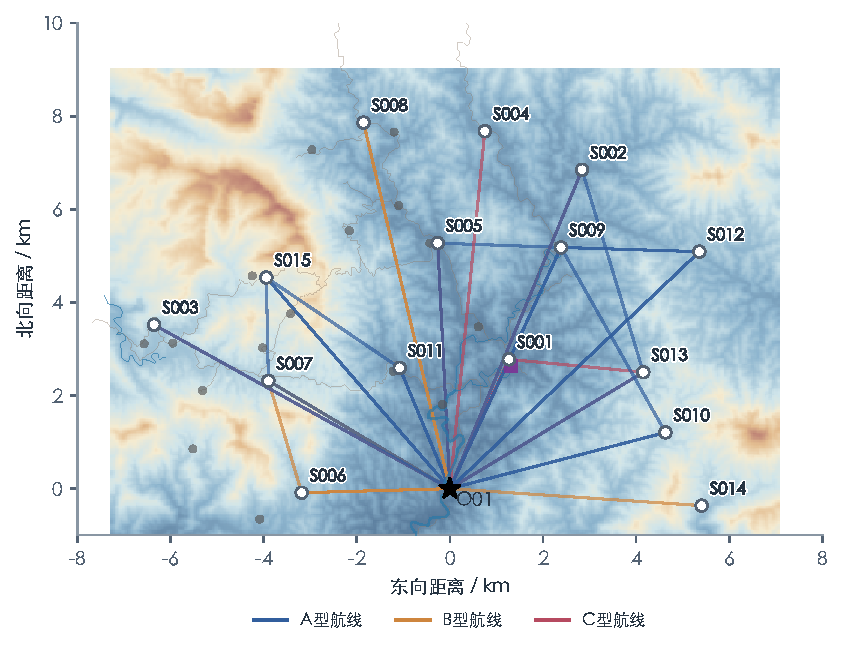
\includegraphics[width=.82\textwidth]{../figures/paper_full_20260926/q2_transport_routes.pdf}\caption{当前24架次方案的多点运输航线}\label{fig:routes}\end{figure}
\begin{figure}[H]\centering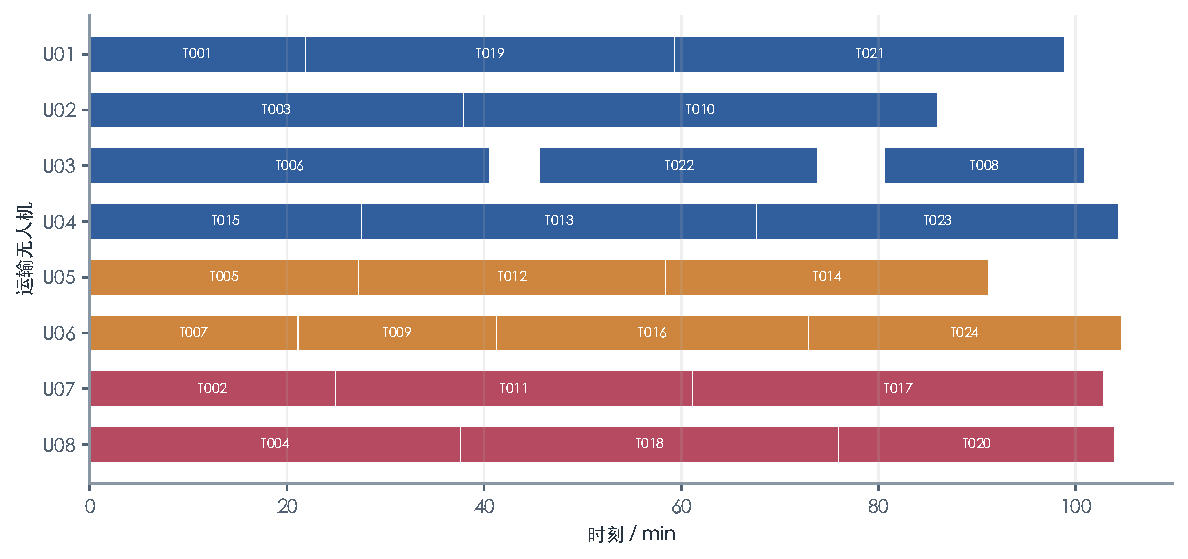
\includegraphics[width=.88\textwidth]{../figures/paper_full_20260926/q2_drone_timeline.pdf}\caption{当前方案的运输机排程}\label{fig:gantt}\end{figure}
\begin{figure}[H]\centering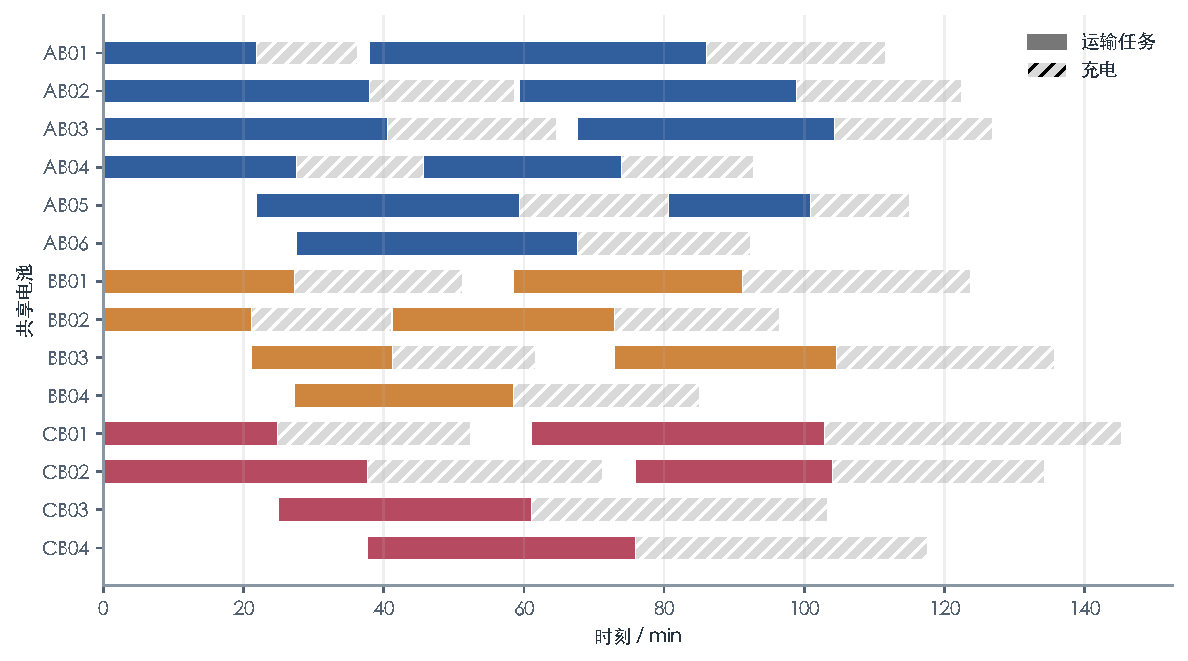
\includegraphics[width=.88\textwidth]{../figures/paper_full_20260926/q2_battery_timeline.pdf}\caption{当前方案的运输电池占用与充电区间}\label{fig:q2_battery}\end{figure}
\begin{figure}[H]\centering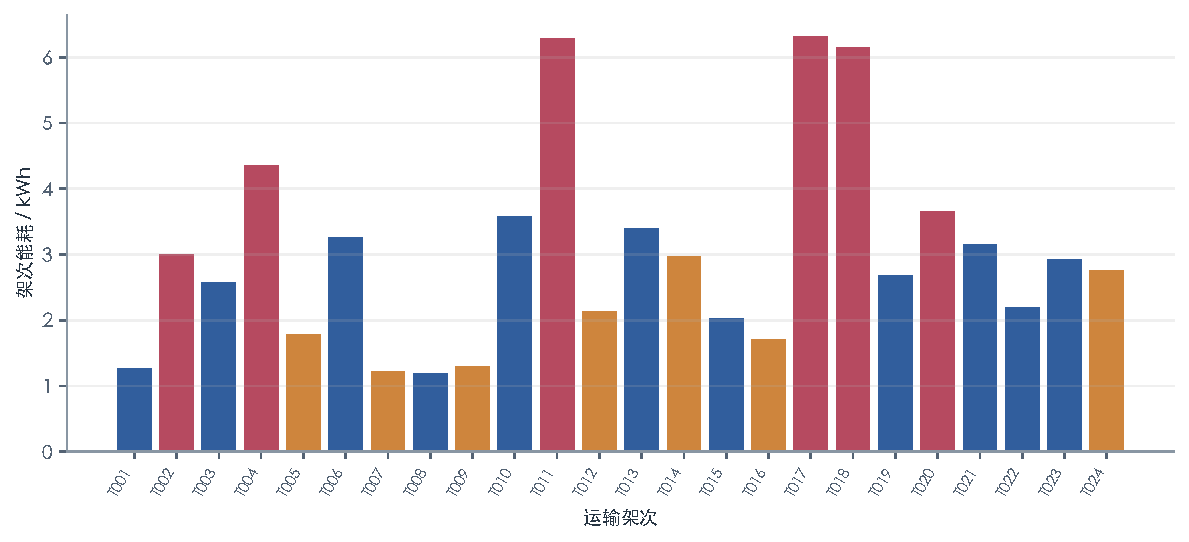
\includegraphics[width=.90\textwidth]{../figures/paper_full_20260926/q2_route_energy.pdf}\caption{当前方案的逐航次能耗}\label{fig:q2energy}\end{figure}
\begin{figure}[H]\centering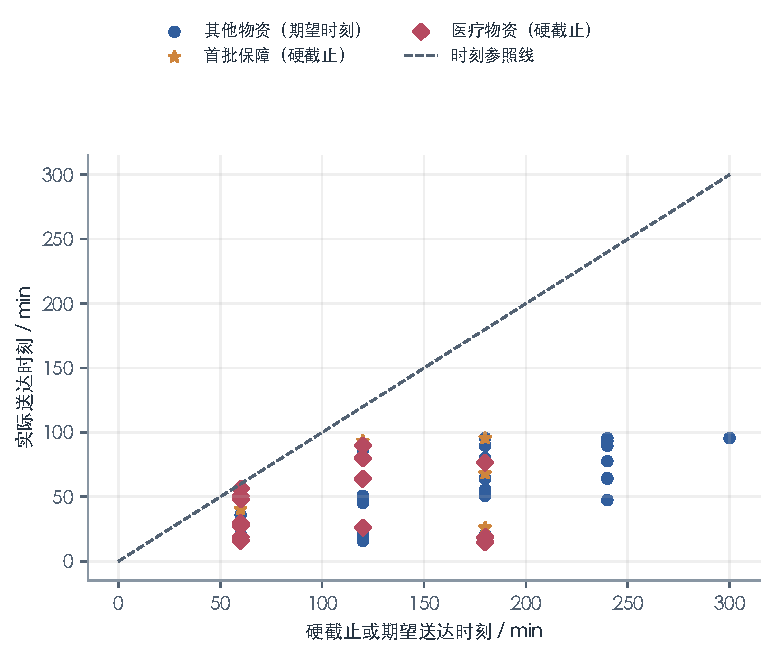
\includegraphics[width=.78\textwidth]{../figures/paper_full_20260926/q2_delivery_deadlines.pdf}\caption{80个货箱的实际送达时刻与时限对照}\label{fig:q2_deadline_plot}\end{figure}
\begin{figure}[H]\centering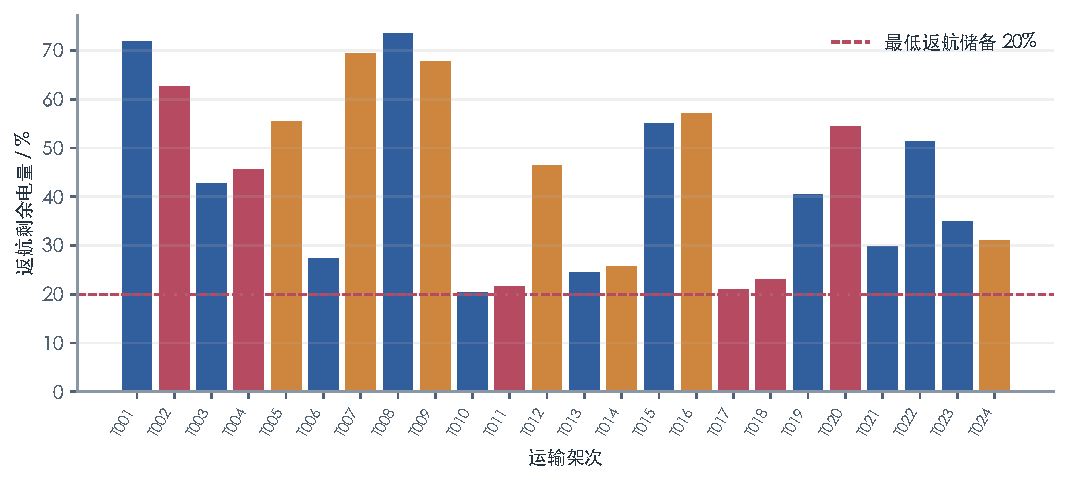
\includegraphics[width=.92\textwidth]{../figures/paper_full_20260926/q2_return_soc.pdf}\caption{当前方案逐架次返航剩余电量}\label{fig:q2_soc}\end{figure}

$\bar{L}_\pi=0$说明64箱非医疗物资均不晚于各自期望时刻，同时31箱硬截止货箱全部满足约束。最小能源裕度$\gamma_E=0.004065$由架次T010决定：该A型机路线为S010$\to$S009$\to$S005，共运送3箱，耗电约3.582~kWh，返航SOC为20.41\%，仅高于20\%下限0.4065个百分点。因此该方案在标称参数下可行，但最紧架次的能源余量较小。问题一的累计作业时间是各单点架次时长之和，问题二的收尾时间是并行调度的最后返航时刻，二者物理含义不同，本章不作数值上的直接比较。

主方案接受三类独立检查：逐航段复算飞行时间、逐段扣重能耗、交接时刻和返航SOC；将货箱分配、载重、体积、能量和硬截止逐项代回约束；检查机体与电池占用及充电区间是否重叠。全部检查通过，程序实现中的人工智能工具辅助情况见参考文献\cite{codexai}和\hyperref[app:ai]{附录~B}。

\subsection{本问小结与适用范围}

问题二在问题一的物理模型上加入多站访问、实体机、电池和配送时限，形成路线生成与资源调度的分层求解框架。最终保留的24架次方案完成80箱投送，满足31箱硬截止和全部资源周转约束，非医疗物资加权迟到为0。该方案是经独立回代验证的可行方案，不是完整路线组合空间的全局最优解。

上述结论限于当前路线邻域、10个种子、每次30个有效候选及给定时间保护。设备性能采用附件标称值，未考虑风场、临时禁飞区和交接工位容量变化；启发式搜索在不同运行环境下也不保证重新产生同一候选。问题三以该24架次方案为运输起点，并为满足连续通信约束调整运输结构、机型和任务时序，同时增加中继保障。因此，问题三相对问题二的架次数、收尾时间和总能耗差额反映运输调整与中继保障共同形成的综合代价，不能归因于单一因素。
